\documentclass[10pt,a4paper]{article}

%Set Margin
\usepackage[left=1in,right=1in,top=1in,bottom=1in]{geometry}

% Support Korean
\usepackage{kotex}
\usepackage{indentfirst}

% Support line spacing
\usepackage{setspace}

% Support Simplied Mathematical Notation by Il-Kyuk-Pil-Sal
\usepackage{ikps}

%===========================================================
% Support Code Example 
\usepackage{listings}
\lstset{frame=tb,
	language=C++,
	aboveskip=3mm,
	belowskip=3mm,
	captionpos=b,
	showstringspaces=false,
	basicstyle=\normalsize,  % 2019 소스 글자크기 조정 함
	numbers=left,
	stepnumber=5,  % 점프 사이즈
	showstringspaces=false,
	tabsize=1,
	breaklines=true,
	breakatwhitespace=false,
	columns=flexible,
	basicstyle={\normalsize\ttfamily},
	numberstyle=\small\color{blue},
	keywordstyle=\color{blue},
	commentstyle=\color{teal},
	stringstyle=\color{magenta},
	breaklines=true,
	breakatwhitespace=true,
	tabsize=3
}

%============================================================
% Support Korean title of contents
\renewcommand{\contentsname}{\center차\hspace*{12pt}례}
\renewcommand{\lstlistingname}{소스코드}
\renewcommand{\lstlistlistingname}{\center소스코드 목차}
\renewcommand{\figurename}{그림}
\renewcommand{\refname}{참고문헌}

%============================================================
% Support PNU Rules about thesis
%============================================================


%=============================================================
% Information of Documents
\title{\textbf{동적계획법을 이용한 유전자 염기서열의 유사성 찾기}}
\author{ 김현수(201424442) \\[3mm]
		 부산대학교 공과대학 정보컴퓨터공학전공 \\[3mm]
		 \textit{alcatra@pusan.ac.kr}
	   }
%==============================================================


\begin{document}
\begin{spacing}{1.6}
\maketitle 
\tableofcontents

\section{서론}
  이 과제는 유전자의 두 염기서열을 분석하여 두 염기서열 중에서 나타날 수 있는 유사한 sequence를 모두 찾는 문제이다. 이 문제는 Local Alignment로 풀어야 하므로 Smith-Waterman Algorithm을 이용하여 풀 수 있다. 
  
\section{Smith-Waterman Algorithm의 활용}
  Smith-Waterman Algorithm[1]은 두 문자열 사이의 Local Alignment를 찾아내는 가장 대표적인 알고리즘으로, Dynamic Programming을 이용하여 찾아내는 방법이다. Dynamic Programming을 위해서는 이전 자료에 대한 일정한 계산값이 존재해야 하고, 이를 이용하여 계산할 자료에 대한 결과를 낼 수 있다. 이를 위하여 이전 자료들을 저장하는 작업을 구현하여야 하는데, 이러한 작업을 Memoization이라 한다. 

\subsection{입력 파일 분석}
  Memoization을 구현하는 방법을 고려하기 위하여 입력파일의 크기를 살펴봤더니, 입력파일에서 받아들여야 하는 문자의 수가 최소 200만 자에 육박하였다. (pa2-test1.fasta) 따라서 배열을 이용하는 방법으로는 메모리를 아껴가며 Memoization을 할 수 없으므로, Memoization을 위한 파일(dp.dat)을 생성한 뒤, 결과를 낸 후에는 삭제하는 것으로 하였다. 

\subsection{풀이}
    먼저, Smith-Waterman Algorithm에 따라, 다음과 같이 두 수열을 비교한 후 Memoization한다. Memoization 배열을 $M$이라 하고, 첫번째 입력파일로부터 받아오는 문자열을 $R$, 두 번째 파일로부터 받아오는 문자열을 $C$라고 하자. 그리고 각각의 index들을 $i,j$라 하면 수식 \ref{e1},\ref{e2}로 결정한다. 다만, $i=0$ 또는 $j=0$인 경우에는 0으로 하고, 첫 글자에 대한 index는 1부터 시작한다. 
    \begin{equation}
    Memoization[i][j] = maximum \begin{cases} 
    	0,\\
    	Memoization[i][j-1] + gap (insertion gap), \\
    	Memoization[i-1][j] + gap (deletion gap),\\
    	Memoization[i-1][j-1] + match(i,j) (match or mismatch)
    	\end{cases}
    	\label{e1}
    \end{equation}
    
    \begin{equation}
    	match(i,j) = \begin{cases} 3&( R[i]=C[j] )\\ -2&( R[i] \neq C[j] ) \end{cases}
    \label{e2}
    \end{equation}
	 
    이 때, 요구사항에 주어진 gap 점수는 -5점만 적용하였고, local alignment에서 sequence를 추출하는 과정에서 반영하였다.(첨부된\texttt{PA02.cpp}를 참조하라.)
    
    Memoization이 끝나면, 가장 높은 점수이면서 가장 뒤의 위치부터 Back-Trace를 수행하여 local alignment를 구한다. 
    
    그림 \ref{f1}은 두 문자열 \texttt{TTATAGTAAG}와 \texttt{ATCCGCTAGG}를 입력받아 Memoization한 예시이다.
    \begin{figure}
    	\centering
    	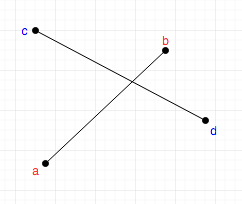
\includegraphics[scale=1]{Fig1.png}
    	\caption{두 문자열 \texttt{TTATAGTAAG}와 \texttt{ATCCGCTAGG}를 입력받아 Memoization하여 나타난 Array 예시, \texttt{TTATAGTAAG}을 이용하여 열을 구성하고,\texttt{ATCCGCTAGG}을 이용하여 행을 구성함.}
    	\label{f1}
    \end{figure}

    Smith-Waterman Algorithm에 따르면, 가장 점수를 많이 받은 9행 6열(9점)부터 Back-Tracing을 수행한다. 그러나, Backtracing의 방향을 정하는 것은 해당 행과 열에 해당하는 문자를 일일이 비교하여야 하므로 계산량이 많아진다. 따라서, 점수를 정한 근거가 무엇인지에 따라(어떤 경우가 최댓값인지에 따라) BackTracing 방향을 정하는 Flag를 수식 \ref{e3}과 같이 부여하였다. 
    \begin{equation}
    	Memoization[i][j] =\begin{cases} 
    	1 (insertion gap), \\
    	2 (deletion gap),\\
    	3 (Memoization[i-1][j-1] + match(i,j)) (match or mismatch)
    	-1 (otherwise)
    	\end{cases}
    	\label{e3}
    \end{equation}
    
    그렇다면, Flag까지 부여하여 나타낸 것은 그림 \ref{f2}과 같고, Back-Tracing의 과정을 살핀다. 
    \begin{figure}
    	\centering
    	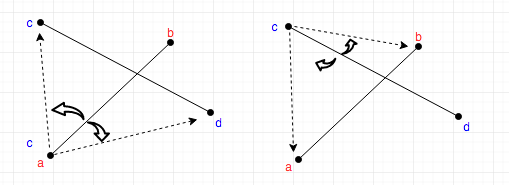
\includegraphics[width=\linewidth]{Fig2.png}
    	\caption{두 문자열 \texttt{TTATAGTAAG}와 \texttt{ATCCGCTAGG}를 입력받아 Memoization하여 나타난 Array 예시 : Flag 부여}
    	\label{f2}
    \end{figure}
    9행6열의 점수가 가장 높고, 가장 뒤에 위치하고 있으므로 시작점으로 한다. 9행6열의 Flag값은 3이므로, 대각선 방향으로 이동한다. 따라서, 8행 5열로 이동한다. 
    다음은 8행 5열을 살핀다. 8행 5열의 Flag값은 3이므로, 역시 대각선 방향인 7행 4열로 이동한다. 7행 4열의 Flag값 역시 3이므로 6행 3열로 이동한다. 6행 3열의 Flag값이 -1이므로, Back-Tracing을 종료한다. 이를 나타낸 것은 \ref{f3}과 같고, 노란색으로 음영처리된 부분은 Back-Tracing이 진행되는 부분, 파란색으로 음영처리된 부분은 Back-Tracing을 종료하는 부분이다.
    \begin{figure}
    	\centering
    	\includegraphics[width=\linewidth]{Fig3.png}
    	\caption{Back-Tracing 예시}
    	\label{f3}
    \end{figure}
    
\section{시간복잡도 분석}
  2의 풀이에 대한 시간복잡도를 분석한다. 풀이에서 수행하는 기본 동작은 크게 Memoization과 Memoization한 자료를 활용하여 BackTracing하는 것으로 나눌 수 있다. 
  
  소스코드 \ref{c1}는 Memoization을 구현한 것으로, $n$의 byte의 길이를 가진 문자열과 $m$의 길이를 가진 문자열에 대하여 각각 1회씩 동작하여 Memoization 배열의 모든 원소를 계산하여 채우고 있으므로, $(m+1) \times (n+1) = mn$의 시간이 걸린다.  $ m \rightarrow N, n \rightarrow N$이면, $(m+1)(n+1) \rightarrow  N^2$이다. 한편,\[ \lim_{N \rightarrow \infty } \dfrac{N^2}{N^2} = 1\] 이므로, $(m+1)(n+1) \in \Theta(N^2)$이다. 
  \begin{lstlisting}[caption={Memoization의 구현, 26번째 줄부러 36번째 줄까지는 점수를 계산하는 작업이고, 그 이후는 Memoization을 위하여 파일에 점수와 Flag를 쓰는 작업이다.}, label={c1}]
  	 private void dynamic_programming::scoring() {
  		this->file.open("dp.dat", ios::out|ios::in|ios::binary);
  		
  		/*
  		* Making Data object for dynamic Programming
  		*  - Calculate Value of cell in memoization table according to Smith-Waterman Algorithm.
  		*/
  		function<_dp_data*(char *)> max_and_flagging = [&](char* _data) -> _dp_data* {
  			char _score = max( max( _data[0], _data[3] ), max(_data[1], _data[2]));
  			char _flag = -1;
  			if (_score == _data[1])
  			_flag = 1;
  			else if (_score == _data[2])
  			_flag = 2;
  			else if (_score == _data[3])
  			_flag = 3;
  			_dp_data *res = new _dp_data(_score,_flag);
  			return res;
  		};
  		
  		if (file.is_open()) {
  			/*
  			* Core of Dynamic Programming
  			*/
  			
  			// basic operation
  			for (size_t i = 1; i<=row ; i++) {
  				for (size_t j = 1; j<=col ; j++ ) {
  					char _cases[4] = {
  						0, // not tagged, terminate
  						at(i,j-1)->getscore() + static_cast<char>(gap),   // insertion gap
  						at(i-1,j  )->getscore() + static_cast<char>(gap), // deletion  gap
  						at(i-1,j-1)->getscore() + \
  						( row_data[i-1] == col_data[j-1] ? static_cast<char>(matched) : static_cast<char>(mismatched) ) // match or mismatch
  					};
  			// end of basic operation
  			
  					_dp_data *_data = max_and_flagging(_cases);
  					
  					// Pin to start of back-tracing for make local alignment
  					if ( _data->getscore() > this->maxscore) {
  						this->maxscore = _data->getscore();
  						this->maxc = j;
  						this->maxr = i;
  					}
  					
  					const char *_data_p = _data->pack();
  					
  					//memoization
  					file.seekp(((i*(col+1))+(j))*3, ios::beg);
  					file.write(_data_p,3);
  					
  					//clean temp-objects for protect from memory corruption.
  					delete _data;
  					delete _data_p;
  					
  				}

  \end{lstlisting}
  다음은, BackTrace를 수행하는 동작을 살핀다. Baktracing의 최악의 상황은 Memoization 배열의 끝부분부터 대각선으로 움직아는 경우(입력된 모든 문자열이 일치하는 경우) 일 것이므로, 배열의 행의 수 만큼이다. 따라서, Backtracing의 시간복잡도는 $\Theta(N)$이다.
  이외, Subsequence를 모두 찾고 점수를 부여하는 과정은 vector를 이용하여 모든 원소에 대하여 계산을 수행하므로 시간복잡도는 $\Theta(N)$이다.
  
  따라서, 2의 풀이의 시간복잡도는 $\Theta(N^2)+\Theta(N)+\Theta(N) \in \Theta(N^2)$ 이다.

\section*{참고문헌}
\noindent[1] Wikipedia, https://en.wikipedia.org/wiki/Smith-Waterman$\_$algorithm

\end{spacing}
\end{document}
